\begin{wrapfigure}{r}{0.41\linewidth}
    \vspace{-28pt}
    \begin{minipage}[t]{0.18\textwidth}
        \begin{minted}{julia}
            y .= 0
            for j = _, i = _
              y[i] += A[i, j] * x[j]
            end
        \end{minted}
        \vspace{24pt} % Add this to ensure top alignment within minipage
        \begin{minted}{julia}
            y .= 0
            for j = _, i = _
              y[j] += A[i, j] * x[i]
            end
        \end{minted}
    \end{minipage}\hfill%
    \begin{minipage}[t]{0.22\textwidth}
        \vspace{0pt} % Add this to ensure top alignment within minipage
        \begin{minted}{julia}
            y .= 0
            for j = _
              let x_j = x[j]
                y_j .= 0
                for i = _
                  let A_ij = A[i, j]
                    y[i] += x_j * A_ij
                    y_j[] += A_ij * x[i]
                  end
                end
                #D is the diagonal
                y[j] += y_j[] + D[j] * x_j
              end
            end
        \end{minted}
    \end{minipage}
    \vspace{-8pt}
    \caption{Finch row-major, column-major and symmetric SpMV Programs}
    \label{spmv_programs}
    \vspace{-12pt}
  \end{wrapfigure}
  \subsection{Sparse Matrix-Vector Multiply (SpMV)}
  Sparse matrix-vector multiplication (SpMV) has a wide range of applications and has been thoroughly studied~\cite{liu_csr5_2015,
  zhou_enabling_2020}. 
  %
  Because SpMV is bandwidth bound, many formats have
  been proposed to reduce the footprint~\cite{langr_evaluation_2016}. 
  %
  The wide range of applications unsurprisingly
  results in a wide range of array structures, making it an effective kernel to
  demonstrate the utility of our programming model. 
  %
  We varied both the data formats and the SpMV algorithm. 
  %
  Our formats
  are shown in Table~\ref{spmv_tensor_formats}, and our programs are listed in
  Figure~\ref{spmv_programs}.
  %
  In varying the program, we consider both row and column-major SpMV programs, as
  well as a symmetric SpMV. 
  %
  Finch enables us to exploit symmetry
  effectively.
  %
  Our program restricts our attention to the canonical triangle (using
  masks), reuses the reads to the canonical triangle of the symmetric matrix
  (using a $\finchdefine$ statement), and writes the results to both relevant
  locations (using multiple outputs).
  %
  All of our programs apply to all of our level formats, enabling exploitation of multiple structural patterns concurrently (e.g. sparsity \textit{and} symmetry).
  
  Figure~\ref{fig:spmv_grouped} displays speedup relative to TACO, SuiteSparseGraphBLAS, and Julia’s standard library.  We test using sparse matrices from a large selection of datasets spanning several previous papers: the datasets used by Vuduc et al. to test the OSKI interface \cite{vuduc2005oski}, Ahrens et al. to test a variable block row format partitioning strategy \cite{ahrens_optimal_2021}, and Kjolstad et al. to test the TACO library \cite{kjolstad_tensor_2017}. Additionally, we included the SNAP graph collection to test with boolean matrices. We also created some synthetic matrices containing bands of varying sizes.
  % or blocks of varying sizes as well as a permutation matrix to encapsulate a few additional use cases.
  %The dense vector is randomly generated. 
  %
  We tested using the row-major and column-major Finch programs in Figure \ref{spmv_programs} as well as the symmetric program where applicable; the performance displayed for Finch on each dataset is the fastest among the formats and programs we tested. For TACO, Column-major SpMV consistently performs better than row-major SpMV (an average of 1.36x better) so we use column-major SpMV in TACO as our baseline.
  
  We found that the SpMV performance was superior for the level format that best paralleled the structure of the tensor.
  %
  Namely, matrices with a clear blocked structure like exdata\_1, TSOPF\_RS\_b678\_c1, and heart3 performed notably well with the SparseVBL format with speedups of 2.16, 1.55, and 1.30 relative to TACO, while the baseline format had slowdowns of 0.71, 0.53, and 0.92 relative to TACO.
  %
  Furthermore, the synthetic banded matrices we constructed performed the best with the SparseBand matrix, in particular with the large\_band and the medium\_band matrices having a speedup of 1.98 and 1.64 relative to TACO, while the baseline format had slowdowns of 0.84 and 0.51 relative to TACO.
  %
  There were also significant advantages of using the Pattern format instead of the Element format to represent scalar values in the matrices when these values were boolean, such as matrices in the SNAP collection which represent graph datasets are boolean. 
  %
  For example, the SparseList-Pattern for email-Eu-core resulted in a speedup of 2.51, while the SparseList-Element format resulted in a slowdown of 1.84 over TACO.
  %
  Every symmetric matrix in the SparseList and SparseList-Pattern formats has better performance when we use a Finch SpMV program that takes advantage of this symmetry.
  %
  Symmetric SpMV with the SparseList level format in Finch results in an average of 1.27x speedup over TACO and symmetric SpMV with the SparseList-Pattern format in Finch results in an average speedup of 1.21x over TACO.
  %
  Notably, there is a 1.91x speedup for the HB/saylr4 matrix over TACO. 
  
  %We consider the Dense(SparseList(Element)) format with the column-major SpMV program to be the Finch baseline as it is the closet analog to the sparse matrix format and SpMV program in other libraries.  
  
  
  %\subsubsection{Tensor Formats}
  
  
  %\subsubsection{Symmetric SpMV}
  % Every symmetric matrix in the SparseList and SparseList-Pattern formats has better performance when we use a Finch SpMV program that takes advantage of this symmetry.
  %However, the regular row- or column-major Finch SpMV programs have better performance for symmetric matrices than the symmetric Finch SpMV program for the other more specialized formats, likely because we need in-order accesses to fully capitalize on the specialized storage.
  
  % \begin{wrapfigure}{r}{0.41\linewidth}
  %     \begin{minipage}[t]{0.18\textwidth}
  %         \vspace{0pt} % Add this to ensure top alignment within minipage
  %         \begin{minted}{julia}
  %             y .= 0
  %             for j = _, i = _
  %               y[i] += A[i, j] * x[j]
  %             end
  %         \end{minted}
  %         \vspace{24pt} % Add this to ensure top alignment within minipage
  %         \begin{minted}{julia}
  %             y .= 0
  %             for j = _, i = _
  %               y[j] += A[i, j] * x[i]
  %             end
  %         \end{minted}
  %     \end{minipage}\hfill%
  %     \begin{minipage}[t]{0.22\textwidth}
  %         \vspace{0pt} % Add this to ensure top alignment within minipage
  %         \begin{minted}{julia}
  %             y .= 0
  %             for j = _
  %               let x_j = x[j]
  %                 y_j .= 0
  %                 for i = _
  %                   let A_ij = A[i, j]
  %                     y[i] += x_j * A_ij
  %                     y_j[] += A_ij * x[i]
  %                   end
  %                 end
  %                 #D is the diagonal
  %                 y[j] += y_j[] + D[j] * x_j
  %               end
  %             end
  %         \end{minted}
  %     \end{minipage}
  %     \vspace{-8pt}
  %     \caption{Finch row-major, column-major and symmetric SpMV Programs}
  %     \label{spmv_programs}
  %     \vspace{-12pt}
  % \end{wrapfigure}
  
  \begin{table}[htbp]
      \scriptsize
      \centering
      \vspace{-12pt}
      \caption{SpMV Tensor Formats}
      \vspace{-12pt}
      \label{spmv_tensor_formats}
      \begin{tabular}{|l|l|l|l|}
          \hline
          \textbf{Outer Level} & \textbf{Inner Level} & \textbf{Scalar Values} & \textbf{Style of Matrix}\\
          \hline
          \multirow{6}{*}{Dense} & \multirow{2}{*}{SparseList} & Element & sparse, real-valued matrices \\
          \cline{3-4} 
          & & Pattern & sparse, boolean-valued matrices \\
          \cline{2-4} 
          & SparseVBL & Element & real-valued matrices with blocked structure \\
          \cline{2-4}
          & SparseBand & Element & real-valued matrices with diagonal band \\
          \cline{2-4}
          & \multirow{2}{*}{SparsePoint} & Element & real-valued matrices with one value per row \\
          \cline{3-4} 
          & & Pattern & matrix with runs of true or false \\
          \hline 
      \end{tabular}
      \vspace{-8pt}
  \end{table}
  
  % Perhaps add the following section again in a future iteration of paper
  % \subsubsection{4D Blocked SpMV}
  % Finch also provides us the capability of writing an SpMV kernel [point to figure] that computes the output in blocks. Specifically, we rewrite an n x n matrix as a n/b x n/b x b x b 4-dimensional tensor and the vector as an n x n/b matrix where b is the block-size. We represent the blocked matrix with a SparseList as its second level (i.e. of format Dense(SparseList(Dense(Dense(Element(0.0)))))) so that only the non-zero blocks are stored. Then, we perform SpMV on each b x b block individually. Note that although SparseVBL already stores consecutive nonzeros in blocks, the benefit of a 4D-blocked kernel is that it additionally computes the output block by block. This method enables us to take advantage of spatial and temporal locality via register reuse [cite].
  
  % We evaluated the 4D-blocked kernel on the Kronecker product of a neural network matrix (erdos-renyi, with sparsity p = ?) with a blocked matrix of size 10x10 and a dense and randomly generated vector. We found a 1.04x speedup to TACO, indicating comparable performance, and a 1.35x speedup to computing a non-blocked SpMV with the SparseVBL format, the fastest performing 2D Finch format for this matrix. 
  
  % Structured matrices with induced dense blocks of equivalent size commonly arise in machine learning applications. In feature extraction, the Kronecker product of image data and a smaller matrix is computed to extract relevant features [cite]. Graph adjacency matrices or Laplacian matrices may also exhibit dense blocks when certain subsets of nodes or edges are densely interconnected. For instance, the adjacency matrix of the Erdös-Renyi random graph has a real symmetric bxb random block at each non-vanishing entry [cite]. 
  
  
  %Here's a figure with spmv_performance_sorted_(faster_than_taco).png and spmv_performance_sorted_(slower_than_taco).png
  
  \begin{figure}
      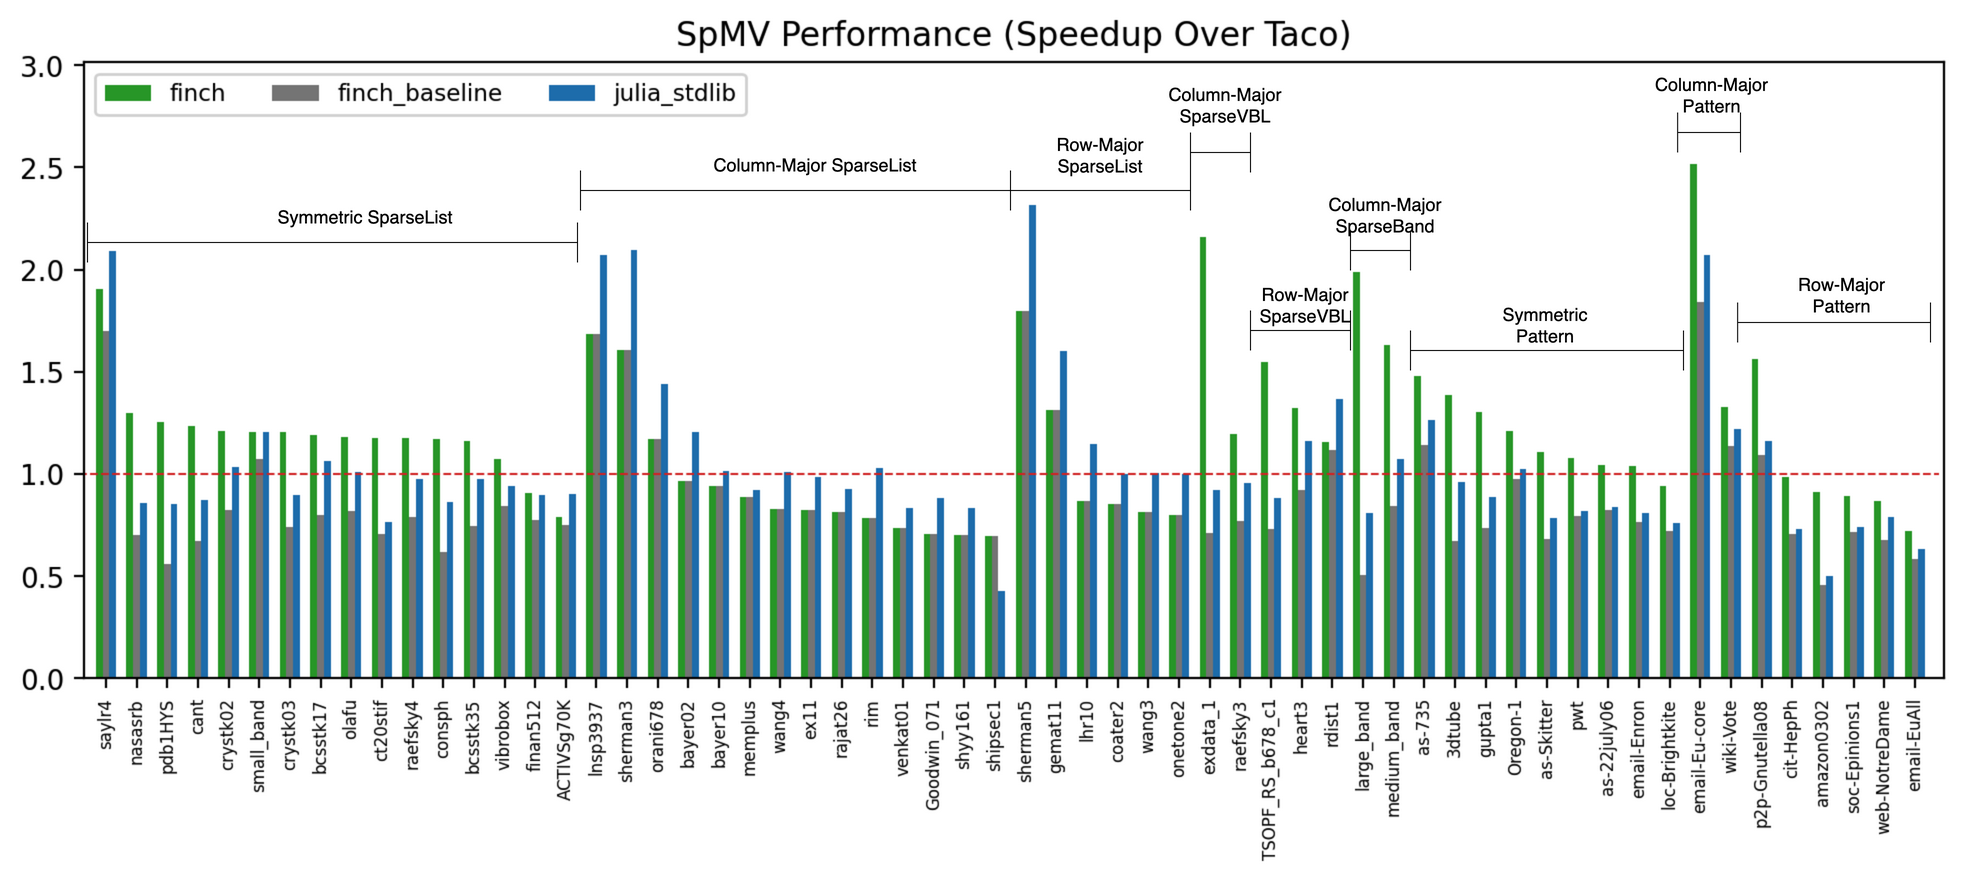
\includegraphics[width=\linewidth]{Spmv_annotated.png}
      \vspace{-18pt}
      \caption{Performance of SpMV by Finch format.}
      \label{fig:spmv_grouped}
      \footnotesize The performance displayed for Finch on each dataset is the fastest among the formats we tested. "R" indicates row-major implementation and "C" indicates column-major implementation in Finch. The baseline Finch format is unsymmetric Dense(SparseList(Element)).
  \end{figure}